\documentclass[border=3pt]{standalone}
% Preâmbulo compartilhado pelos diagramas TikZ da aula 8 de IHR (Métodos de Pesquisa)
\usepackage[T1]{fontenc}
\usepackage[utf8]{inputenc}
\usepackage{lmodern}
\usepackage{amsmath}
\usepackage{xcolor}
\usepackage{tikz}
\usetikzlibrary{arrows.meta,angles,quotes,decorations.pathmorphing,decorations.pathreplacing,calc,
                positioning,shapes.geometric,shapes.misc,backgrounds,fit,
                math}

% Paleta (mesma dos SVGs originais)
% Paleta da disciplina de IHR: acento azul (#1A6FB5), cor de destaque do tema.
% (o nome "dblue" é mantido para não alterar todos os diagramas)
\definecolor{dblue}{HTML}{1A6FB5}
\definecolor{dorange}{HTML}{B3541E}
\definecolor{dgreen}{HTML}{4A7C59}
\definecolor{dred}{HTML}{9C4B4B}
\definecolor{dcream}{HTML}{F4F1EA}
\definecolor{dshade}{HTML}{DDD7C9}

% Função gaussiana (não normalizada por padrão de escala visual)
\pgfmathdeclarefunction{gauss}{3}{%
  \pgfmathparse{1/(#3*sqrt(2*pi))*exp(-((#1-#2)^2)/(2*#3^2))}%
}

% Estilos comuns (prefixo d... para não colidir com chaves internas do pgf)
\tikzset{
  >={Stealth[length=2mm]},
  dguide/.style={gray!55, dashed, line width=0.4pt},
  daxis/.style={gray!60, line width=0.7pt, ->},
  dbody/.style={fill=black!3, draw=black!80, line width=1pt},
  dacc/.style={draw=dblue, line width=1pt},
  dlbl/.style={black!55, font=\small},
  dsub/.style={black!45, font=\footnotesize},
  dstate/.style={circle, draw=black!80, fill=dcream, line width=1pt,
                 minimum size=17mm, font=\large, inner sep=1pt},
  dobs/.style={circle, draw=black!80, fill=dshade, line width=1pt,
               minimum size=14mm, font=\large, inner sep=1pt},
  dbox/.style={rounded corners=2pt, draw=black!80, fill=dcream, line width=1pt,
               align=center, inner sep=6pt},
  dop/.style={circle, draw=black!80, fill=white, line width=1pt,
              minimum size=6mm, inner sep=0pt, font=\small},
  dtrans/.style={->, dblue, line width=1pt},
  dmeas/.style={->, dorange, line width=1pt},
  dcurve/.style={line width=1pt, dblue},
  dcurveb/.style={line width=1.4pt, dorange},
}

\begin{document}
\hyphenpenalty=10000 \exhyphenpenalty=10000 \tolerance=9999 \emergencystretch=3em
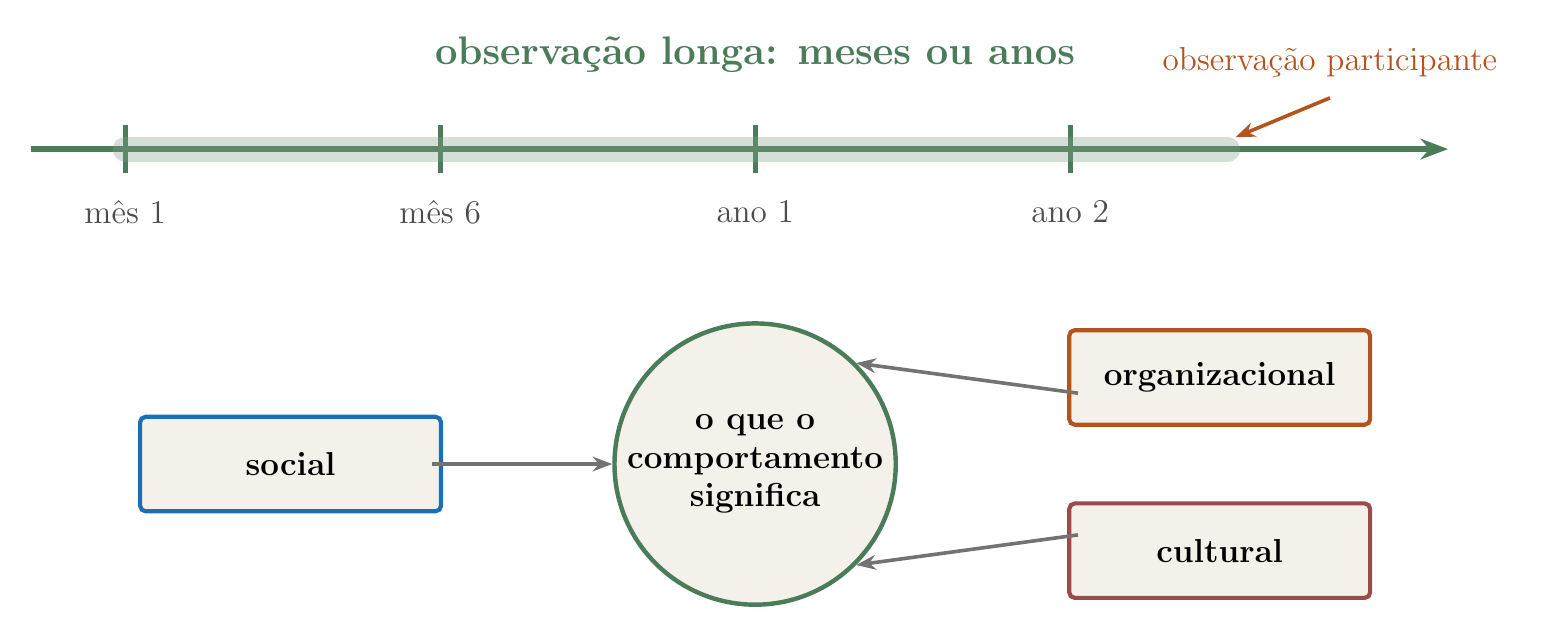
\begin{tikzpicture}[x=1cm,y=1cm]
  \draw[dgreen, line width=2.2pt, -{Stealth[length=3.5mm]}] (0.3,7.2) -- (18.3,7.2);
  \foreach \x/\t in {1.5/{mês 1},5.5/{mês 6},9.5/{ano 1},13.5/{ano 2}} {\draw[dgreen, line width=1.8pt] (\x,6.9) -- (\x,7.5); \node[font=\large, black!70] at (\x,6.4) {\t};}
  \draw[dgreen!70, line width=9pt, opacity=0.35, line cap=round] (1.5,7.2) -- (15.5,7.2);
  \node[font=\Large\bfseries, dgreen] at (9.5,8.4) {observação \textbf{longa}: meses ou anos};
  \node[font=\large, dorange, text width=4.5cm, align=center] at (16.8,8.3) {observação participante};
  \draw[dorange, line width=1.3pt, -{Stealth[length=2.5mm]}] (16.8,7.85) -- (15.6,7.35);
  \node[dstate, minimum size=3.1cm, font=\large\bfseries, align=center, draw=dgreen, line width=1.6pt] (c) at (9.5,3.2) {o que o\\ comportamento\\ significa};
  \node[dbox, draw=dblue, line width=1.5pt, text width=3.4cm, minimum height=1.2cm, font=\large\bfseries] at (3.6,3.2) {social};
  \node[dbox, draw=dorange, line width=1.5pt, text width=3.4cm, minimum height=1.2cm, font=\large\bfseries] at (15.4,4.3) {organizacional};
  \node[dbox, draw=dred, line width=1.5pt, text width=3.4cm, minimum height=1.2cm, font=\large\bfseries] at (15.4,2.1) {cultural};
  \draw[black!55, line width=1.3pt, -{Stealth[length=2.5mm]}] (5.4,3.2) -- (c.west);
  \draw[black!55, line width=1.3pt, -{Stealth[length=2.5mm]}] (13.6,4.1) -- (c.north east);
  \draw[black!55, line width=1.3pt, -{Stealth[length=2.5mm]}] (13.6,2.3) -- (c.south east);
\end{tikzpicture}
\end{document}
